\documentclass[12pt,a4paper]{article} 
\usepackage{tikz}
\usepackage{float}
\usepackage{graphicx}
\usepackage{multirow}
\usepackage{setspace} 
\usepackage{graphicx}
\usepackage{times}
\pagenumbering{roman}
\usepackage{geometry}

\geometry{verbose,tmargin=2cm,bmargin=2cm,lmargin=3cm,rmargin=2cm}
\usepackage{fancyhdr} 
%\linespread{1.05} 
\usepackage{tikz}
\usetikzlibrary{arrows}
\usetikzlibrary{shapes.geometric}

\tikzstyle{kres} = [rectangle, rounded corners, minimum width=1cm, minimum height=0.5cm,text centered, draw=black]
\tikzstyle{nad} = [trapezium, trapezium left angle=60, trapezium right angle=100, minimum width=1cm, minimum height=0.5cm, text centered, draw=black]
\tikzstyle{sim} = [trapezium, trapezium left angle=60, trapezium right angle=100, minimum width=1cm, minimum height=0.5cm, text centered, draw=black]
\tikzstyle{garis} = [thick,->,>=stealth]
\usetikzlibrary{shapes,arrows}

\begin{document} % Mulai Penulisan Laporan
\onehalfspacing
\begin{titlepage}

\title{\textbf{LAPORAN PRAKTIKUM ELEKTRONIKA DASAR
\\ HIGH PASS FILTER DAN LOW PASS FILTER}}  %Judul Laporan
%\title{\textbf{FOTOKATALISIS}}  %Judul Laporan
\author{\textbf {Dosen : Mada Sanjaya WS, Ph.D  }
\\ \textbf{Asisten Lab : Sri Rohmawati (1177030037)}
\\ \textbf{ }
\\ \textbf{Disusun Oleh :}
\\ \textbf{Muhamad Fahmi Adzkar} \textbf {(1187030024)}
\\ \textbf{Kelompok 3 :}
\\ \textbf{Hani Hikmawati} \textbf {(1187030014)}
\\ \textbf{Sri Rahayu} \textbf {(1187030036)}
\\ \textbf{Yuni Rahayu} \textbf {(1187030041)}}

\maketitle
\begin{center}
\vspace{1cm}

\includegraphics[width=4cm]{uin.png}
\vspace{1cm}

JURUSAN FISIKA\\
FAKULTAS SAINS DAN TEKNOLOGI\\
UIN SUNAN GUNUNG DJATI BANDUNG\\
2019\\
\end{center}
\end{titlepage}

\renewcommand\abstractname{Abstract} %Untuk Abstrak Bahasa Inggris
\begin{abstract} %Untuk Abstrak Bahasa Inggris
A high-pass filter (HPF) is an electronic filter that passes signals with a frequency higher than a certain cutoff frequency and attenuates signals with frequencies lower than the cutoff frequency. The amount of attenuation for each frequency depends on the filter design. A high-pass filter is usually modeled as a linear time-invariant system. It is sometimes called a low-cut filter or bass-cut filter. High-pass filters have many uses, such as blocking DC from circuitry sensitive to non-zero average voltages or radio frequency devices. They can also be used in conjunction with a low-pass filter to produce a bandpass filter.

In the optical domain, high-pass and low-pass have the opposite meanings, with a "high-pass" filter (more commonly "long-pass") passing only longer wavelengths (lower frequencies), and vice-versa for "low-pass" (more commonly "short-pass").

\textit{Keywords: Capasitor, Resistant, Voltage, GAIN}
\end{abstract}

\begin{abstract}
Sebuah high-pass filter ( HPF ) adalah penyaring elektronik yang melewati sinyal dengan frekuensi yang lebih tinggi daripada tertentu frekuensi cutoff dan attenuates sinyal dengan frekuensi rendah daripada frekuensi cutoff. Jumlah redaman untuk setiap frekuensi tergantung pada desain filter. Filter high-pass biasanya dimodelkan sebagai sistem invarian waktu linier . Kadang-kadang disebut filter berpotongan rendah atau filter bass-cut . Filter high-pass memiliki banyak kegunaan, seperti memblokir DC dari sirkuit sensitif terhadap tegangan rata-rata tidak nol atau perangkat frekuensi radio . Mereka juga dapat digunakan bersama dengan filter low-pass untuk menghasilkan filter bandpass .

Dalam domain optik, high-pass dan low-pass memiliki arti yang berlawanan, dengan filter "high-pass" (lebih umum "long-pass") hanya panjang gelombang yang lebih panjang (frekuensi yang lebih rendah), dan sebaliknya untuk "rendah -pass "(lebih umum" short-pass ").

\textit{Kata Kunci: Kapasitor, Resistansi, Tegangan, GAIN}
\end{abstract}


\newpage
\section{PENDAHULUAN}
\paragraph{1.1 Latar Belakang}
\subparagraph{ }
	Penguat Operasional (Operasional Amplifier) atau yang biasa disebut Op-Amp merupakan suatu jenis penguat elektronika dengan hambatan (coupling) arus searah yang memiliki faktor penguatan sangat besar dengan dua masukan dan satu pengeluaran.
\subparagraph{ }
	Pada umumnya penguat operasional tersedia dalam bentuk sirkuit terpadu dan yang paling banyak digunakan adalah ranfkaian seri. Penguat opersional dalam rangkaian terpadu memiliki karakteristik yang mendekati karakteristik penguat operasional ideal tanpa perlu memperhatikan apa yang terdapat di dalamnya.
\subparagraph{ }
Penguat operasional adalah perangkat yang sangat efisien dan serba guna. Contoh penggunaan penguat operasional adalah untuk operasi matematika sederhana seperti penjumlahan dan pengurangan terhadap tegangan listrik hingga dikembangkan kepada penggunaan aplikatif seperti komparator dan osilator dengan distorsi rendah serta pengembangan alat komunikasi. Selain itu, aplikasi pemakaian op-amp juga meliputi bidang elektronika audio, pengatur tegangan DC, tapis aktif, penyearah presisi, pengubah analog digital dan pengubah digital ke analog, pengolah isyarat seperti cuplik tahan, penguat pengunci, kendali otomatik, computer analog, elektronika nuklir, dan lain-lain.

\paragraph{1.2 Tujuan}
\subparagraph{ }
Adapun tujuan dilakukannya praktikum ini yaitu:
\begin{enumerate}
\item Mampu memahami rangkaian HPF dan LPF.
\item Mampu menganalisa prinsip kerja rangkaian HPF dan LPF.
\item Mengetahui gelombang input dan output pada setiap rangkaian.
\item Dapat menghitung tegangan output dari setiap rangkaian.
\end{enumerate}


\newpage
\section{Landasan Teori}
\subsection{Dasar Teori}
\paragraph{ }
\textbf{1.Penguat operasional}
\subparagraph{ }
 Penguat operasional (bahasa Inggris: operational amplifier) atau yang biasa disebut op-amp merupakan suatu jenis penguat elektronika dengan sambatan (bahasa Inggris: coupling) arus searah yang memiliki bati (faktor penguatan atau dalam bahasa Inggris: gain) sangat besar dengan dua masukan dan satu keluaran.Penguat operasional pada umumnya tersedia dalam bentuk sirkuit terpadu dan yang paling banyak digunakan adalah seri 741.

Penguat operasional adalah perangkat yang sangat efisien dan serba guna.Contoh penggunaan penguat operasional adalah untuk operasi matematika sederhana seperti penjumlahan dan pengurangan terhadap tegangan listrik hingga dikembangkan kepada penggunaan aplikatif seperti komparator dan osilator dengan distorsi rendah.

Penguat operasional dalam bentuk rangkaian terpadu memiliki karakteristik yang mendekati karakteristik penguat operasional ideal tanpa perlu memperhatikan apa yang terdapat di dalamnya.Karakteristik penguat operasional ideal adalah:
\begin{enumerate}
\item Bati tegangan tidak terbatas.
\item Impedansi masukan tidak terbatas.
\item Impedansi keluaran nol.
\item Lebar pita tidak terbatas.
\item Tegangan offset nol (kondisi ketika masukan sebesar nol).
\end{enumerate}
	
\begin{flushright}
(Wikipedia.com)
\end{flushright}

\subparagraph{ }
\textbf{2.Rangkaian High Pass Filter}
\subparagraph{ }
 Filter high-pass elektronik urutan pertama sederhana yang ditunjukkan pada Gambar 1 diimplementasikan dengan menempatkan tegangan input pada kombinasi seri kapasitor dan resistor dan menggunakan tegangan melintasi resistor sebagai output. Produk dari resistensi dan kapasitansi ($ R x C $ ) adalah konstanta waktu ; itu berbanding terbalik dengan frekuensi cutoff f c , yaitu di mana f c adalah di hertz , t dalam detik , R adalah ohm , dan C dalam farad .

Gambar 2 menunjukkan implementasi elektronik aktif dari filter high-pass tingkat pertama menggunakan penguat operasional . Dalam hal ini, filter memiliki gain passband - R 2 / R 1 dan memiliki frekuensi cutoff Karena filter ini aktif , mungkin memiliki gain passband non-unity . Artinya, sinyal frekuensi tinggi dibalik dan diperkuat oleh R 2 / R 1 .

\subparagraph{ }
1. Realisasi waktu-terpisah .
Untuk metode konversi lain dari waktu kontinu ke diskrit, lihat Transformasi Bilinear .
Filter high-pass waktu diskrit juga dapat dirancang. Desain filter waktu diskrit berada di luar cakupan artikel ini; namun, contoh sederhana datang dari konversi filter lintasan tinggi waktu kontinu di atas ke realisasi waktu terpisah. Artinya, perilaku waktu kontinu dapat didiskritisasi .

Dari sirkuit pada Gambar 1 di atas, menurut Hukum Kirchhoff dan definisi kapasitansi :
dimana ${ Q_ {c} (t)}Q_c (t)$ 
 adalah muatan yang disimpan dalam kapasitor pada saat itu ${t}t.$
 Mengganti Persamaan (Q) menjadi Persamaan (I) dan kemudian Persamaan (I) ke Persamaan (V) memberikan:
 
 High Pass Filter atau biasanya disingkat dengan HPF adalah Filter atau penyaring frekuensi yang dapat melewatkan sinyal frekuensi tinggi dan menghambat atau memblokir sinyal frekuensi rendah. Dengan kata lain, sinyal Frekuensi tinggi akan lebih mudah melewati High Pass Filter (HPF) sedangkan sinyal frekuensi rendah akan dihambat atau dipersulit untuk melewatinya. HPF yang ideal adalah HPF yang sama sekali tidak melewatkan sinyal dengan frekuensi dibawah frekuensi cut-off. Pada dasarnya, High Pass Filter (HPF) adalah kebalikan dari Low Pass Filter (LPF). Dalam bahasa Indonesia, High Pass Filter disebut juga dengan Tapis Lolos Tinggi, Tapis Pelewat Tinggi atau Penyaring Lolos Atas.


 
Tapis Lolos Tinggi atau High Pass Filter ini dapat dibuat dengan menggunakan komponen pasif seperti Resistor dengan Kapasitor atau Induktor. High Pass Filter yang dibuat dari Resistor dan Kapasitor disebut dengan High Pass RC Filter sedangkan High Pass Filter atau HPF yang terbuat dari Resistor dan Induktor disebut dnegan High Pass RL Filter. Filter Pasif yaitu filter yang menggunakan komponen pasif ini tidak memiliki elemen penguat seperti Transistor dan Op-Amp sehingga tidak memiliki perolehan penguatan sinyal, oleh karena itu tingkat OUTPUT-nya selalu kurang dari tingkat INPUT-nya.


\subparagraph{ }
2. High Pass RC Filter
High Pass RC Filter atau Penyaring Lolos Atas RC adalah rangkaian penyaring frekuensi yang terdiri dari komponen pasif yaitu Resistor (R) dan Kapasitor (C) yang meneruskan sinyal frekuensi tinggi tetapi menghambat atau memblokir frekuensi rendah. Untuk membuat Penyaring RC ini, Kapasitor (C) ditempatkan secara seri dengan sinyal INPUT rangkaian dan Resistor (R) ditempatkan secara paralel atau sejajar dengan sinyal INPUT seperti yang ditunjukan pada gambar dibawah ini :

Dari rangkaian High Pass RC Filter diatas, Kapasitor (C) yang merupakan komponen reaktif ini akan menawarkan resistansi yang berbeda terhadap sinyal frekuensi yang berbeda yang masuk melaluinya. Resistansi Kapasitor akan tinggi terhadap sinyal frekuensi rendah atau sinyal DC sedangkan resistansi rendah terhadap sinyal frekuensi tinggi. Karena dengan karakteristik kapasitor yang beresistansi tinggi terhadap sinyal frekuensi rendah atau sinyal DC, Kapasitor tersebut akan menghalangi sinyal frekuensi rendah untuk melewatinya sehingga hanya sinyal frekuensi tinggi saja yang berhasil melewati kapasitor tersebut. Kapasitor jenis ini juga berfungsi sebagai Kapasitor kopling (Coupling Capasitor) karena melewatkan sinyal AC tetapi memblokir sinyal DC.

High Pass Filter merupakan penyaring frekuensi yang banyak digunakan diberbagai jenis rangkaian, salah satunya adalah rangkaian Mikrofon. Mikrofon adalah perangkat yang memerlukan daya DC agar dapat beroperasi dan membutuhkan sinyal AC seperti suara manusia dan musik sebagai sinyal INPUT-nya. Dengan kata lain, sinyal DC hanya sebagai daya agar dapat mengoperasikan mikrofon namun tidak boleh muncul pada OUTPUT yang bersinyal AC (Audio). Jadi, untuk meneruskan sinyal Audio yang berbentuk sinyal AC dan memblokir sinyal DC, kita memerlukan rangkaian High Pass Filter (HPF) atau Penyaring Lolos Atas.

\subparagraph{ }
3. High Pass RL Filter
High Pass RL Filter adalah High Pass Filter yang terdiri dari Resistor dan Induktor yang dapat meneruskan sinyal Frekuensi Tinggi tetapi melemahkan atau memblokir sinyal frekuensi rendah. Untuk merangkaian Rangkaian High Pass RL Filter ini, Induktor ditempatkan secara paralel dengan sinyal sumber daya yang memasuki rangkaian sedangkan Resistor ditempatkan secara seri dengan sinyal INPUTnya seperti yang ditunjukan pada gambar dibawah ini:

Rangkaian diatas adalah rangkaian High RL Filter yang dapat melewati sinyal frekuensi tinggi dan melemahkan sinyal frekuensi rendah. Sama seperti Kapastior, Induktor juga merupakan komponen reaktif yang dapat berubah resistansi-nya tergantung pada sinyal frekuensi yang melaluinya. Induktor akan melewati sinyal frekuensi rendah dengan resistansi yang rendah sedangkan frekuensi tinggi yang melalui akan dihambat atau dilemahkan dengan resistansi yang tinggi. Dengan demikian, sinyal frekuensi rendah akan mudah melewati Induktor sedangkan sinyal frekuensi tinggi akan dilemahkan atau diblokir sebagai OUTPUT pada rangkaian High Pass Filter ini.

Rangkaian diatas menggunakan prinsip kerja Reaktansi Induktif. Perlu diingat bahwa arus akan mengambil jalur yang resistansinya paling rendah. Karena Induktor menawarkan resistansi yang tinggi terhadap sinyal frekuensi tinggi, sinyal frekuensi tinggi tidak akan melalui Induktor dan akan mengambil jalur alternatif yang menawarkan resistansi rendah, yaitu jalur ke OUTPUT pada rangkaian RL Filter ini. Di satu sisi, sinyal frekuensi rendah akan melewati jalur ke Induktor karena Induktor menawarkan resistansi yang rendah untuk sinyal frekuensi rendah.

\begin{flushright}
(Wikipedia.com) 
\end{flushright}

\paragraph{ }
\textbf{3. Rangkaian Low Pass Filter}
\subparagraph{ }
	Low Pass Filter atau sering disingkat dengan LPF adalah Filter atau Penyaring yang melewatkan sinyal Frekuensi rendah dan menghambat atau memblokir sinyal Frekuensi tinggi. Dengan kata lain, LPF akan menyaring sinyal frekuensi tinggi dan meneruskan sinyal frekuensi rendah yang diinginkannya. Sinyal yang dimaksud ini dapat berupa sinyal listrik seperti sinyal audio atau sinyal perubahan tegangan. LPF yang ideal adalah LPF yang sama sekali tidak melewatkan sinyal dengan frekuensi diatas frekuensi cut-off (fc) atau tegangan OUPUT pada sinyal frekuensi diatas frekuensi cut-off sama dengan 0V. Dalam bahasa Indonesia, Low Pass Filter ini sering disebut dengan Penyaring Lolos Bawah atau Tapis Pelewat Rendah.
Baca juga : Pengertian Frekuensi dan Cara Menghitung Frekuensi.


 
Penyaring Lolos Bawah atau Low Pass Filter ini dapat dibuat dengan menggunakan beberapa macam komponen pasif seperti Resistor dan Kapasitor atau Induktor. Low Pass Filter yang dibuat dengan Resistor dan Kapasitor disebut dengan Low Pass RC Filter sedangkan Low Pass Filter yang dibuat dengan Resistor dan Induktor disebut dengan Low Pass RL Filter. Filter yang hanya menggunakan komponen pasif ini sering disebut dengan Filter Pasif, Filter Pasif ini tidak memiliki elemen penguat seperti Transistor dan Op-Amp sehingga tidak memiliki perolehan penguatan sinyal, oleh karena itu tingkat OUTPUT-nya selalu kurang dari tingkat INPUT-nya.

Dua Jenis Konfigurasi Utama Low Pass Filter

Seperti yang disebutkan sebelumnya, terdapat dua konfigurasi utama pada Low Pass Filter Pasif atau Penyaring Lolos Bawah Pasif ini yaitu Low Pass RC Filter (Resistor-Capasitor) dan Low Pass RL Filter (Resistor-Induktor). Berikut ini adalah pembahasan singkat mengenai kedua konfigurasi Low Pass Filter Pasif ini.

\subparagraph{ }
1. Low Pass RC Filter.
Low Pass RC Filter atau Penyaring Lolos Bawah RC ini adalah rangkaian filter yang terdiri dari dari komponen pasif Resistor dan Kapasitor yang meneruskan sinyal frekuensi rendah dan memblokir sinyal frekuensi tinggi. Untuk membuat Low Pass RC Filter, Resistor ditempat secara seri ke sinyal INPUT dan Kapasitor ditempatkan sejajar atau Paralel dengan sinyal INPUT seperti ditunjukan pada gambar dibawah ini :

Dengan rangkaian Low Pass RC Filter diatas, Kapasitor yang merupakan perangkat reaktif ini akan menawarkan resistansi yang berbeda terhadap sinyal frekuensi yang berbeda yang masuk melaluinya. Resistansi pada Kapasitor akan sangat tinggi apabila dilewati oleh sinyal frekuensi rendah atau DC dan resistansi akan menjadi rendah apabila dilewati oleh sinyal frekuensi tinggi. Dengan demikian,  Kapasitor akan memblokir sinyal frekuensi rendah atau sinyal DC sehingga sinyal tersebut harus melewati atau diteruskan ke jalur alternatif yang ditunjukan oleh arah panah pada gambar diatas. Sedangkan sinyal frekuensi tinggi akan melewati Kapasitor karena kapasitor menawarkan resistansi yang rendah bagi sinyal frekuensi tinggi tersebut.

Perlu diingat bahwa arus akan selalu mengambil jalur yang resistansinya paling rendah, karena kapasitor menawarkan resistansi yang rendah dalam rangkaian frekuensi tinggi maka mereka akan akan mengambil jalur melalui kapasitor. Sementara sinyal frekuensi rendah akan mengambil jalur alternatif dengan resistansi yang lebih rendah.

\subparagraph{ }
2. Low Pass RL Filter
Low Pass RL Filter atau Penyaring lolos bawah RL adalah rangkaian penyaring frekuensi yang terdiri dari komponen Resistor dan Induktor yang melewati atau meneruskan Frekuensi rendah dan memblokir atau menghambat frekuensi tinggi. Untuk membuat Low Pass RL Filter, Induktor ditempatkan secara seri dengan sinyal INPUT dan Resistor ditempatkan sejajar atau paralel dengan sinyal INPUT seperti pada gambar rangkain dibawah ini :

Cara kerja rangkaian Low Pass RL Filter diatas berdasarkan prinsip Reaktansi Induktif. Reaktansi Induktif adalah resistansi atau impedansi Induktor yang berubah berdasarkan sinyal frekuensi yang melewatinya. Tidak seperti Resistor yang merupakan perangkat non-reaktif, Induktor menawarkan Impedansi yang berbeda untuk sinyal frekuensi yang berbeda, seperti halnya kapasitor. Namun resistansi yang dihasilkan oleh Induktor ini merupakan kebalikan dari Kapasitor, Resistansi Induktor akan menjadi sangat tinggi apabila dilewati sinyal frekuensi tinggi dan sebaliknya akan menjadi rendah apabila dilewati frekuensi rendah. Oleh karena itu, penempatan Induktor di rangkaian berbeda dengan penempatan Kapasitor pada rangkaian RC Filter.

Berdasarkan karakteristik ini, rangkaian RL (Resistor Induktor) diatas dapat berfungsi secara efektif sebagai Penyaring Lolos Bawah atau Low Pass Filter yang memblokir sinyal frekuensi tinggi dan memungkinkan sinyal frekuensi rendah melewatinya tanpa hambatan.
	
\begin{flushright}
(Wikipedia.com) 
\end{flushright}

\newpage
\section{METODE PRAKTIKUM}
\subsection{Waktu dan Tempat}
\paragraph{ }
Praktikum ini dilaksanakan pada:
\\ 		Tanggal : jum'at, 13 Desember 2019
\\ 		Waktu : 07.00 WIB - Selesai
\\ 		Tempat : Advance Physics 


\subsection{Alat dan Bahan}
Alat dan bahan yang digunakan dalam praktikum ini diantaranya adalah : 
\subparagraph*{ }
\begin{tabular}{|l|l|l|}  \hline
No & Alat dan Bahan  & Jumlah  \\ \hline
1  & Projek board & 1 Buah \\ \hline
2  & IC LM741 & satu set \\ \hline
3  & Baterai 9 volt & Secukupnya \\ \hline
4  & Kancing Baterai 3 Pin & 1 Buah \\ \hline
5  & Kabel Tunggal  & Secukupnya \\ \hline
6  & Resistor  & 2 Buah \\ \hline
7  & Multimeter & Satu set \\ \hline
8  & Osiloskop & Satu set \\ \hline
\end{tabular}

  
    
\subsection{Prosedur Percobaan}
\subparagraph{3.3.1 Percobaan Rangkaian High Pass Filter }
\subparagraph{ }
\textbf{Rangkaian High Pass Filter} Rangkaian disusun sesuai dengan gambar di lampiran dan project board. Kemudian siapkan alat dan bahan yang digunakan. Kemudian Susun rangkaian sesuai dengan gambar simulasi di papan tulis. kemudian ukur besar resistansi pada resistor. Dilanjut dengan diukurnya besar tegangan pada rangkaian inverting dan ketika diberikan tegangan sebesar 9 V arus DC, diukur  V pada rangkaian inverting ketika kondisi stabil di osiloskop. kemudian data ditulis pada tabel.
	
\subparagraph{3.3.2 Percobaan Rangkaian Low Pass Filter }
\subparagraph{ }
	\textbf{Rangkaian Low Pass Filter} Rangkaian disusun sesuai dengan gambar di lampiran dan project board. Kemudian siapkan alat dan bahan yang digunakan. Kemudian Susun rangkaian sesuai dengan gambar simulasi di papan tulis. kemudian ukur besar resistansi pada resistor. Dilanjut dengan diukurnya besar tegangan pada rangkaian inverting dan ketika diberikan tegangan sebesar 9 V arus DC, diukur  V pada rangkaian inverting ketika kondisi stabil di osiloskop. kemudian data ditulis pada tabel.

\subsection{Diagram Alir}
\subsubsection{Percobaan Rangkaian High Pass Filter }
\tikzstyle{line} = [draw, -latex']
\tikzstyle{cloud} = [draw, rectangle,fill=blue!20, node distance=3cm,
    minimum height=0.7cm]
\tikzstyle{kres} = [draw, rectangle, rounded corners,fill=blue!20, node distance=3cm,
    minimum height=0.7cm]
\begin{tikzpicture}[node distance = 1.3cm, auto]
    % Place nodes
       \node [kres] (a) {Siapkan alat dan bahan yang digunakan};
       \node [cloud, below of = a , node distance = 1.5cm] (b) {Susun rangkaian sesuai dengan gambar};         
       \node [cloud, below of = b , node distance = 1.5cm] (c) {Mengukur nilai resistansi pada resistor};
       \node [cloud, below of = c , node distance = 1.5cm] (d) {Masukan tegangan Baterai 9 Volt DC};
       \node [cloud, below of = d , node distance = 1.5cm] (e) {Mengukur V output dengan osiloskop ketika kondisi gelombang stabil};        
       \node [cloud, below of = e , node distance = 1.5cm] (f) {Hasil data ditulis pada tabel};
        
        
     % Draw edges
    \path [line] (a) -- (b);
    \path [line] (b) -- (c);
    \path [line] (c) -- (d);
    \path [line] (d) -- (e);
    \path [line] (e) -- (f);
    \end{tikzpicture}   

	\subsubsection{Percobaan Rangkaian Low Pass Filter }
\tikzstyle{line} = [draw, -latex']
\tikzstyle{cloud} = [draw, rectangle,fill=blue!20, node distance=3cm,
    minimum height=0.7cm]
\tikzstyle{kres} = [draw, rectangle, rounded corners,fill=blue!20, node distance=3cm,
    minimum height=0.7cm]
\begin{tikzpicture}[node distance = 1.3cm, auto]
    % Place nodes
       \node [kres] (a) {Siapkan alat dan bahan yang digunakan};
       \node [cloud, below of = a , node distance = 1.5cm] (b) {Susun rangkaian sesuai dengan gambar};         
       \node [cloud, below of = b , node distance = 1.5cm] (c) {Mengukur nilai resistansi pada resistor};
       \node [cloud, below of = c , node distance = 1.5cm] (d) {Masukan tegangan Baterai 9 Volt DC};
       \node [cloud, below of = d , node distance = 1.5cm] (e) {Mengukur V output dengan osiloskop ketika kondisi gelombang stabil};        
       \node [cloud, below of = e , node distance = 1.5cm] (f) {Hasil data ditulis pada tabel};
        
     % Draw edges
    \path [line] (a) -- (b);
    \path [line] (b) -- (c);
    \path [line] (c) -- (d);
    \path [line] (d) -- (e);
    \path [line] (e) -- (f);
    \end{tikzpicture}   

\newpage

\section{Data dan Pembahasan}

\subsection{Data Hasil Pengamatan}
\paragraph{ } Setelah melakukan eksperimen, maka didapatkan hasil percobaan sebagai berikut.

\subparagraph*{$\bullet$ Rangkaian Percobaan High Pass Filter }
\subparagraph*{ }
\begin{tabular}{|c|c|c|c|c|c|c|c|c|c|c|}        \hline
No & R (HPF) & C (HPF)  & Ri & Rf & F ambang & Fam > Fin   & Gain    \\ \hline 
1. & 560 	 & 1 KmF 	& 1K & 1K & 0,28 Hz  & Lebih Besar & 0,27    \\ \hline
2. & 330 	 & 1 KmF	& 1K & 1K & 0,48 Hz  & Lebih Besar & 0,43  	 \\ \hline
3. & 220	 & 1 KmF 	& 1K & 1K & 0,73 Hz  & Lebih Besar & 0,58 	 \\ \hline
\end{tabular}
 
\subparagraph*{$\bullet$ Rangkaian Percobaan High Pass Filter }
\subparagraph*{ }
\begin{tabular}{|c|c|c|c|c|c|c|c|c|c|c|}        \hline
No &  Vin & Vout (Osiloskop) & Vout (Perhitungan)   		\\ \hline 
1. &  6V  & 0,0015 Volt 	 & 0,0000000672 Volt    		\\ \hline
2. &  10V & 0,0015 Volt 	 & 0,000000190 Volt 			\\ \hline
3. &  10V & 0,0015 Volt 	 & 0,000000285 Volt	 			\\ \hline
 \end{tabular}

\subparagraph*{$\bullet$ Rangkaian Percobaan Low Pass Filter }
\subparagraph*{ }
\begin{tabular}{|c|c|c|c|c|c|c|c|c|c|c|}        \hline
No & R (LPF) & C (LPF)  & Ri & Rf & F ambang & Fam < Fin   & Gain    \\ \hline 
1. & 560 	 & 1 KmF 	& 1K & 1K & 0,28 Hz  & Lebih Kecil & 0,27    \\ \hline
2. & 330 	 & 1 KmF	& 1K & 1K & 0,48 Hz  & Lebih Kecil & 0,43  	 \\ \hline
3. & 220	 & 1 KmF 	& 1K & 1K & 0,33 Hz  & Lebih Kecil & 0,58 	 \\ \hline
\end{tabular}
 
\subparagraph*{$\bullet$ Rangkaian Percobaan High Pass Filter }
\subparagraph*{ }
\begin{tabular}{|c|c|c|c|c|c|c|c|c|c|c|}        \hline
No &  Vin 	   & Vout (Osiloskop) & Vout (Perhitungan)   		\\ \hline 
1. &  0,4 Volt & 0,4 Volt 		  & 0,023 Volt    				\\ \hline
2. &  0,4 Volt & 0,4 Volt 		  & 0,028 Volt 					\\ \hline
3. &  0,4 Volt & 0,4 Volt 		  & 0,031 Volt	 				\\ \hline
\end{tabular}


\newpage
\subsection{Pembahasan}
\subparagraph{ }
	Berdasarkan praktikum yang telah dilakukan, maka dapat diketahui bahwa prinsip kerja IC LM741 pada rangkaian High Pass Filter memiliki dua karakteristik. yaitu jika arus yang masuk melalui Va (negatif) maka akan menjadi penguat pembalik dan pada osiloskop akan memberikan sinyal sinusoidal negatif. Sedangkan sebaliknya, jika arus yang masuk melalui Vb (positif) maka akan menjadi penguat dan pada osiloskop akan memberikan sinyal sinusoidal positif.
	Berdasarkan hasil yang telah dilakukan dengan Hardware. Pada rangkaian percobaan High Pass Filter, didapatkan bahwa Tegangan masuk (Vin) bernilai 6 Volt dan 10 Volt, dan didapatkan bahwa Tegangan keluar (Vout) bernilai 0,0015 Volt (ketika mengamati tegangan di Osiloskop), dan didapatkan bahwa Tegangan keluar (Vout) bernilai 0,0000000672 Volt, 0,000000190 Volt,dan 0,000000285 Volt (ketika mengamati tegangan di perhitungan). Menurut hipotesa praktikan hal tersebut dapat terjadi karena perbedaan resistansi yang cukup jauh . Namun perbedaan nilai arus-arus tersebut tidak terlalu besar yaitu hanya sedikit. Maka dari itu hasil dari praktikum ini hampir sesuai dengan teori hukum Rangkaian High Pass Filter.
\subparagraph{ }
	Berdasarkan hasil yang telah dilakukan dengan Hardware. Pada rangkaian percobaan Low Pass Filter, didapatkan bahwa Tegangan masuk (Vin) bernilai 0,4 Volt, dan didapatkan bahwa Tegangan keluar (Vout) bernilai 0,4 Volt (ketika mengamati tegangan di Osiloskop), dan didapatkan bahwa Tegangan keluar (Vout) bernilai 0,023 Volt, 0,028 Volt,dan 0,031 Volt (ketika mengamati tegangan di perhitungan). Menurut hipotesa praktikan hal tersebut dapat terjadi karena perbedaan resistansi yang cukup jauh . Namun perbedaan nilai arus-arus tersebut tidak terlalu besar yaitu hanya sedikit. Maka dari itu hasil dari praktikum ini hampir sesuai dengan teori hukum Rangkaian Low Pass Filter.
\newpage
 
\subsection{Analisis Data}
\subparagraph{}
	Hasil praktikum ini bisa dinyatakan berhasil tidaknya dapat dilihat dari hasil data, jika besar tegangan (vout) yang dihasilkan tidak beda jauh dan bernilai sama dengan hasil perhitungan teori maka itu dapat dikatakan berhasil. adapun faktor yang mempengaruhi hasil kesalahan-kesalahan pada saat praktikum yaitu pada saat pengolahan data dan juga pada saat pengambilan data pada saat menggunakan alat.
 

\newpage
\section{Kesimpulan}
\subparagraph{ }
Dari praktikum ini dapat disimpulkan bahwa :
\begin{enumerate}

\item Operational Amplifier atau lebih dikenal dengan istilah Op-Amp adalah salah satu dari bentuk IC Linear yang berfungsi sebagai Penguat Sinyal listrik. Sebuah Op-Amp terdiri dari beberapa Transistor, Dioda, Resistor dan Kapasitor yang terinterkoneksi dan terintegrasi sehingga memungkinkannya untuk menghasilkan Gain (penguatan) yang tinggi pada rentang frekuensi yang luas. Dalam bahasa Indonesia, Op-Amp atau Operational Amplifier sering disebut juga dengan Penguat Operasional.

\item Penguat operasional (bahasa Inggris: operational amplifier) atau yang biasa disebut op-amp merupakan suatu jenis penguat elektronika dengan sambatan (bahasa Inggris: coupling) arus searah yang memiliki bati (faktor penguatan atau dalam bahasa Inggris: gain) sangat besar dengan dua masukan dan satu keluaran. Penguat operasional pada umumnya tersedia dalam bentuk sirkuit terpadu dan yang paling banyak digunakan adalah seri 741.
Penguat operasional adalah perangkat yang sangat efisien dan serba guna. Contoh penggunaan penguat operasional adalah untuk operasi matematika sederhana seperti penjumlahan dan pengurangan terhadap tegangan listrik hingga dikembangkan kepada penggunaan aplikatif seperti komparator dan osilator dengan distorsi rendah.

\item Op-Amp umumnya dikemas dalam bentuk IC, sebuah IC Op-Amp dapat terdiri dari hanya 1 (satu) rangkaian Op-Amp atau bisa juga terdiri dari beberapa rangkaian Op-Amp. Jumlah rangkaian Op-Amp dalam satu kemasan IC dapat dibedakan menjadi Single Op-Amp, dual Op-Amp dan Quad Op-Amp. Ada juga IC yang didalamnya terdapat rangkaian Op-Amp disamping rangkaian utama lainnya.

\item Karakteristik Faktor Penguat atau Gain pada Op-Amp pada umumnya ditentukan oleh Resistor Eksternal yang terhubung diantara Output dan Input pembalik (Inverting Input). Konfigurasi dengan umpan balik negatif (Negative Feedback) ini biasanya disebut dengan Closed-Loop configuration atau Konfigurasi Lingkar Tertutup. Umpan balik negatif ini akan menyebabkan penguatan atau gain menjadi berkurang dan menghasilkan penguatan yang dapat diukur serta dapat dikendalikan. Tujuan pengurangan Gain dari Op-Amp ini adalah untuk menghindari terjadinya Noise yang berlebihan dan juga untuk menghindari respon yang tidak diinginkan. Sedangkan pada Konfigurasi Lingkar Terbuka atau Open-Loop Configuration, besar penguatannya adalah tak terhingga $(tak terhingga)$ sehingga besarnya tegangan output hampir atau mendekati tegangan Vcc.

\end{enumerate}

\newpage
\begin{thebibliography}{99} % Daftar Pustaka
\bibitem{1} {Nave, Carl Rod (2006). "HyperPhysics - Operational Amplifier" (dalam bahasa Inggris). Department of Physics and Astronomy, Georgia State University. Diakses tanggal 2010-05-08. }

\bibitem{2} {Terjemahan istilah berdasarkan: "Glosarium". Pusat Bahasa Departemen Pendidikan Nasional. Diakses tanggal 2010-05-08.}

\bibitem{3} {Carter, Bruce; Brown, Thomas. "Handbook of Operational Amplifier Applications" (PDF). Texas Instruments. Diakses tanggal 2010-05-15}

\bibitem{4} {Tipler, Paul A., 1998 ”‘Fisika untuk Sains dan Teknik” .Jakarta : Erlangga }

\end{thebibliography}

\newpage
\begin{center}
\large{\textbf{LAMPIRAN}}
\end{center}

\newpage
\begin{figure}
\paragraph{Gambar perhitungan rumus}
\paragraph{ }
\begin{center}

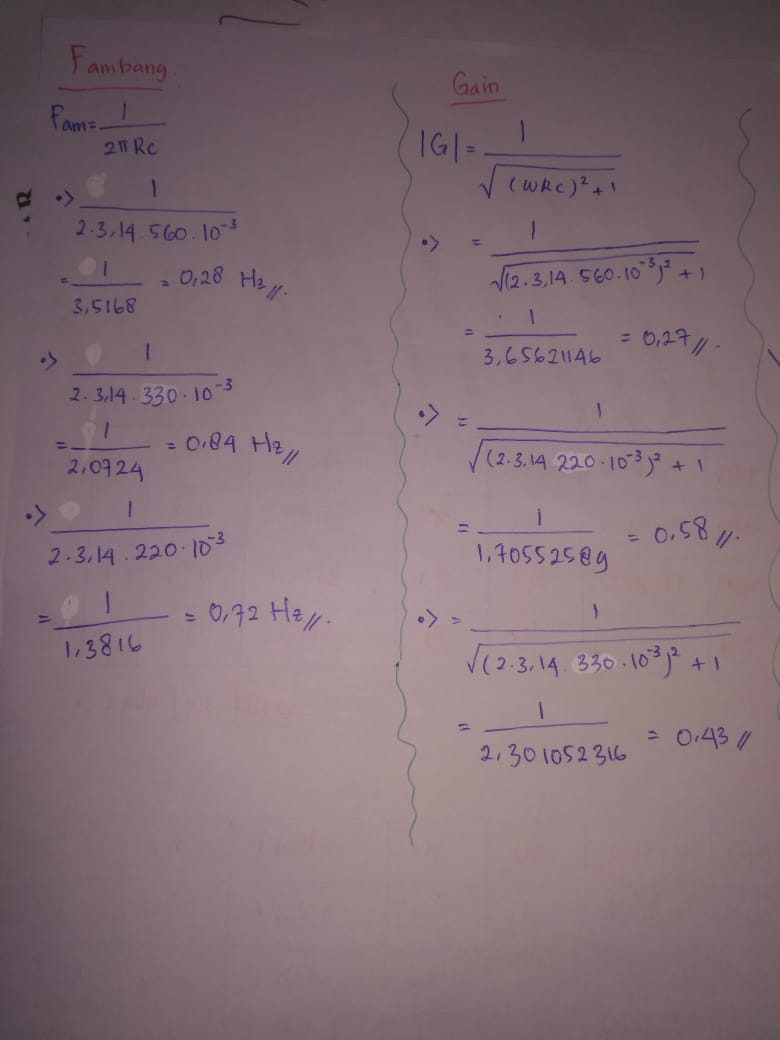
\includegraphics[width=8cm, height=12cm]{Hitung1.png}

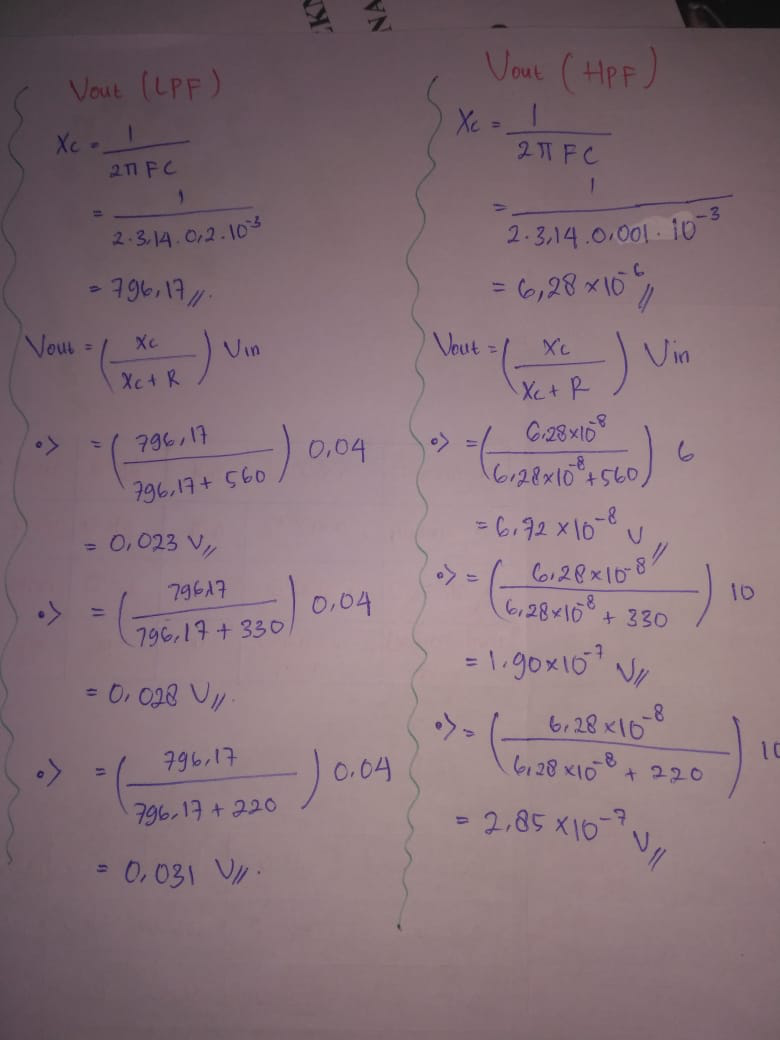
\includegraphics[width=8cm, height=12cm]{Hitung2.png}

\end{center}
\end{figure}
\vspace{2cm}

\newpage
\begin{figure}
\paragraph{Gambar percobaan High Pass Filter}
\paragraph{ }
\begin{center}

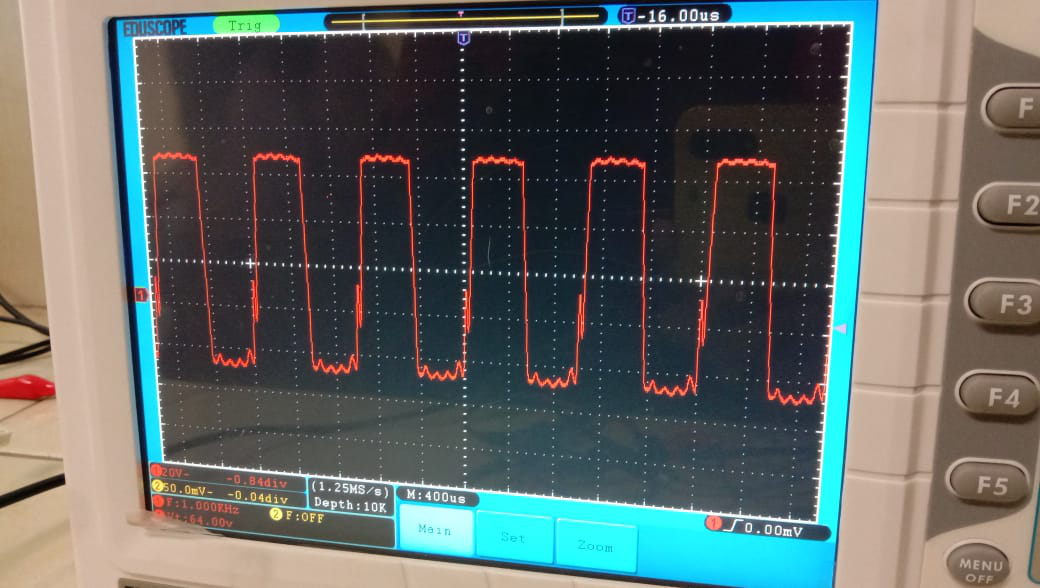
\includegraphics[width=12cm, height=6cm]{HPF1.png}

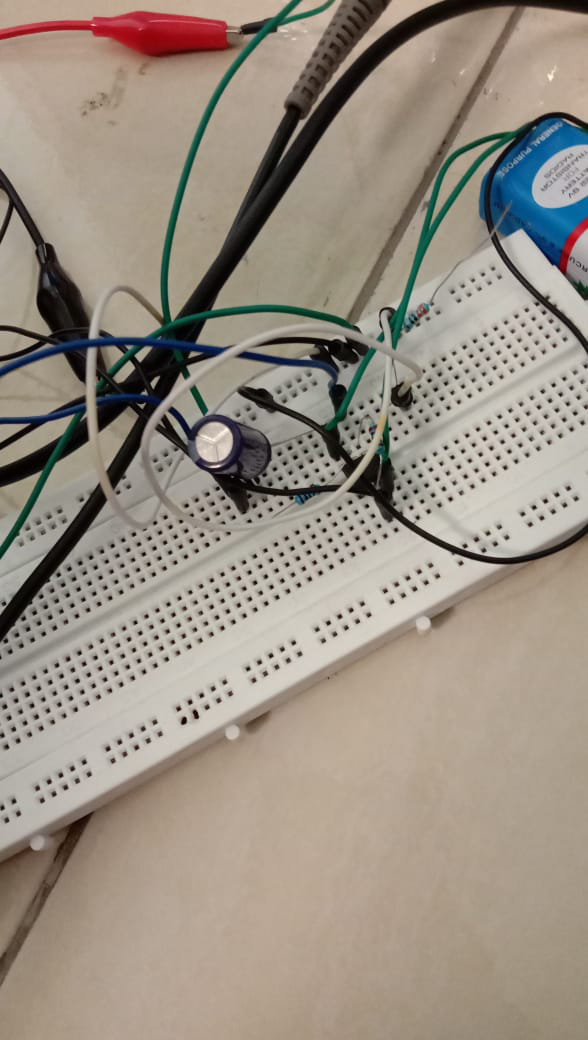
\includegraphics[width=5cm, height=12cm]{HPF2.png}

\end{center}
\end{figure}
\vspace{2cm}

\newpage
\begin{figure}
\paragraph{Gambar percobaan High Pass Filter}
\paragraph{ }
\begin{center}

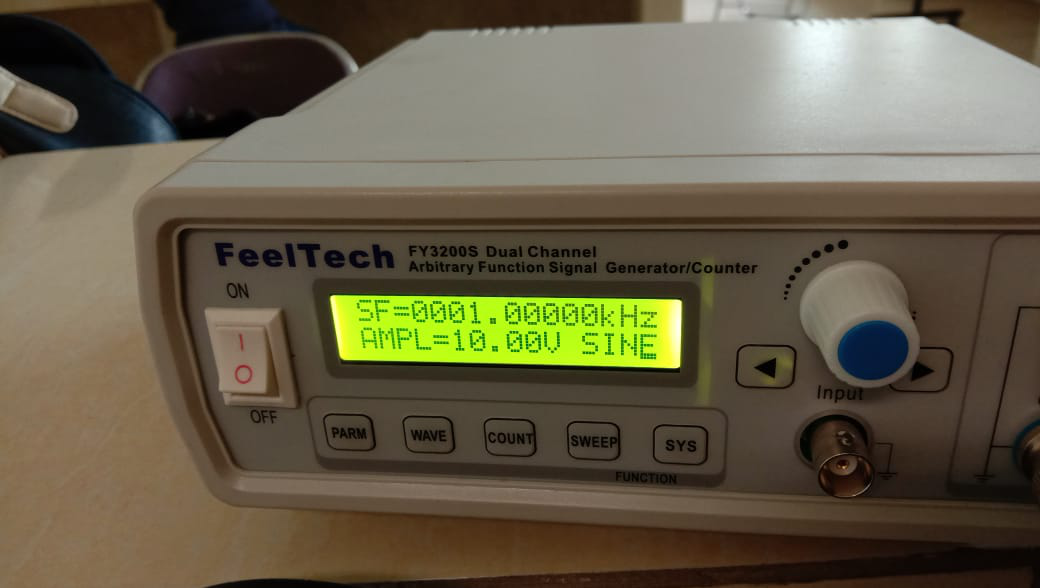
\includegraphics[width=12cm, height=6cm]{HPF3.png}

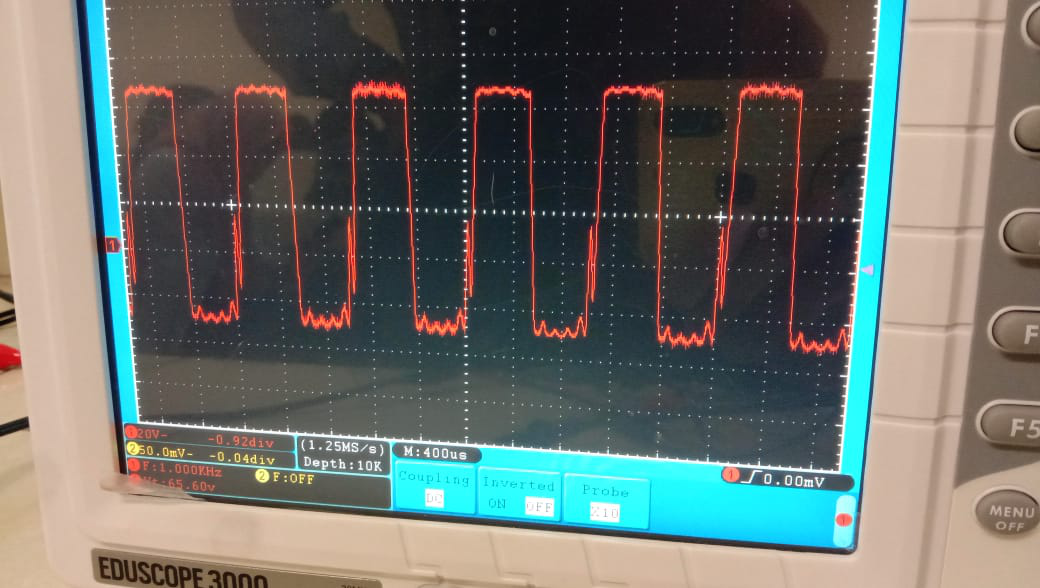
\includegraphics[width=12cm, height=6cm]{HPF4.png}

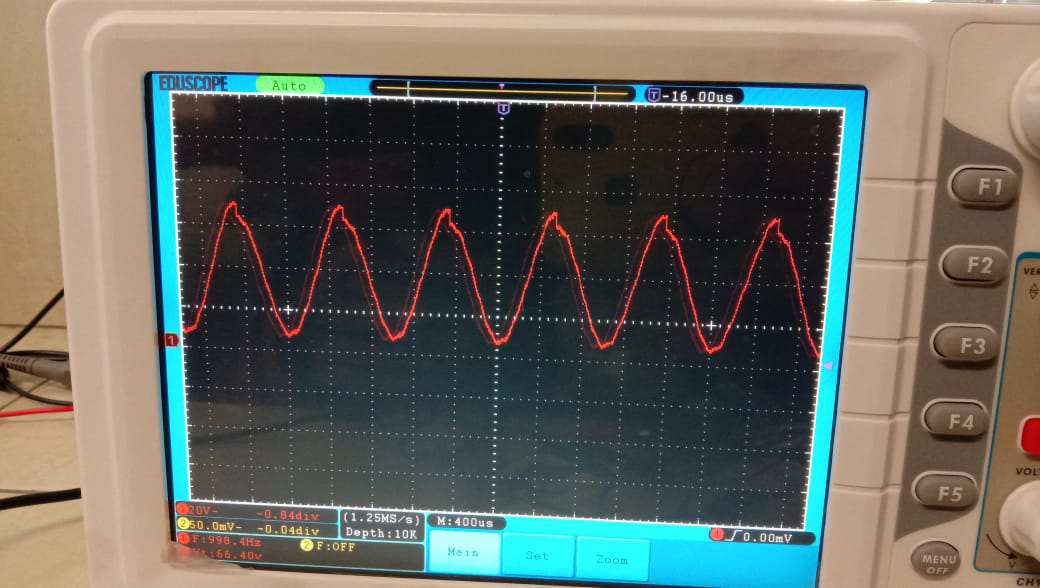
\includegraphics[width=12cm, height=6cm]{HPF5.png}

\end{center}
\end{figure}
\vspace{2cm}

\newpage
\begin{figure}
\paragraph{Gambar percobaan Low Pass Filter dan tabel perhitungan}
\paragraph{ }
\begin{center}

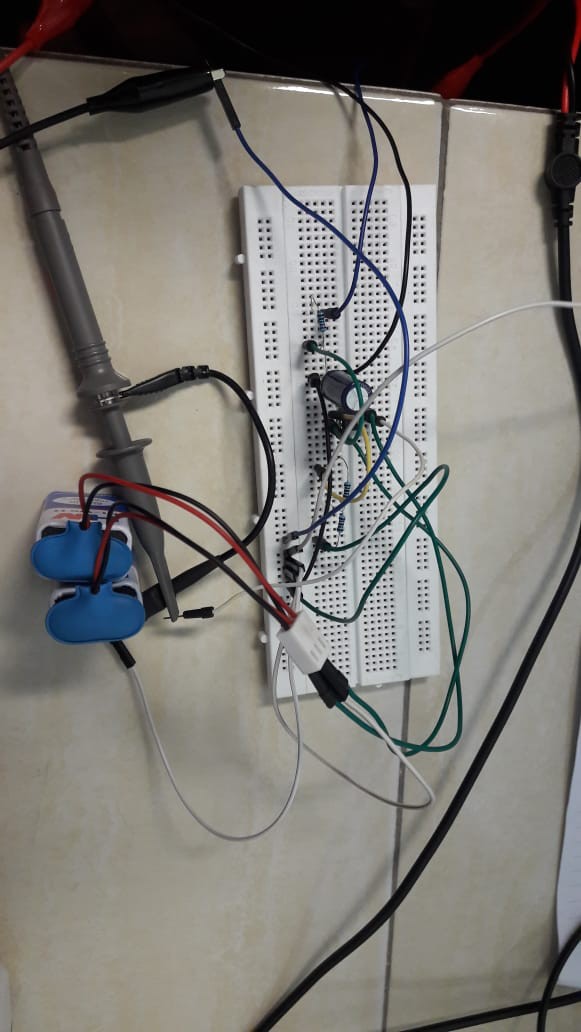
\includegraphics[width=5cm, height=12cm]{LPF1.png}

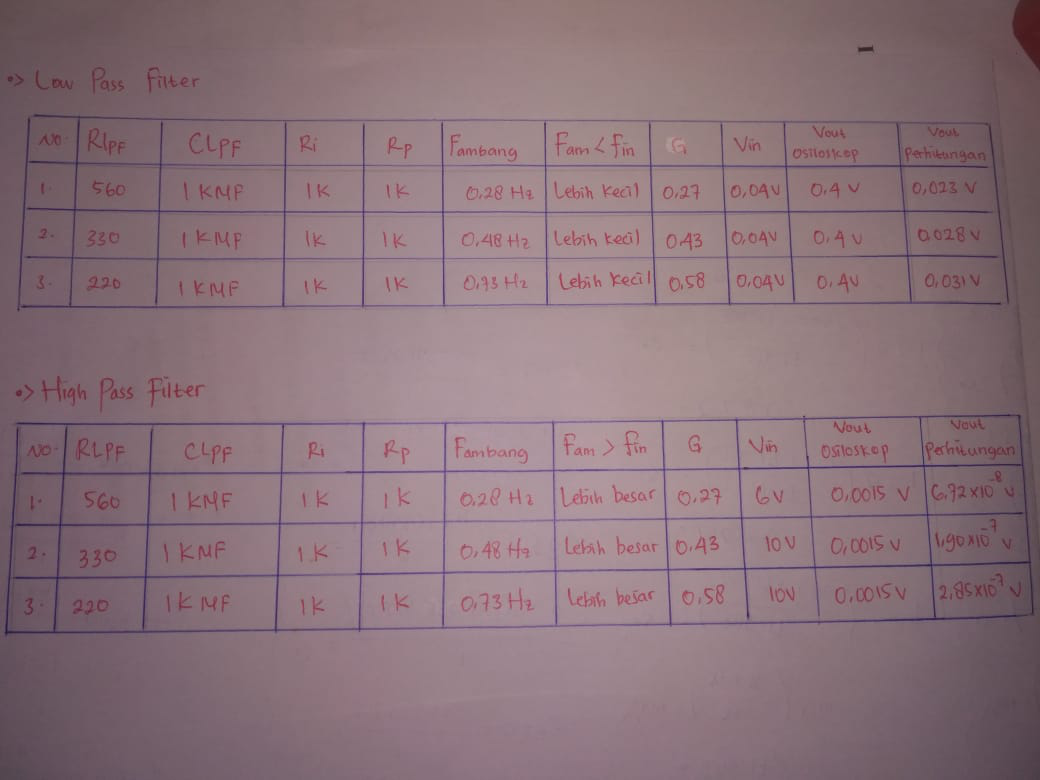
\includegraphics[width=12cm, height=6cm]{Hitung3.png}

\end{center}
\end{figure}
\vspace{2cm}


\end{document} %Penulisan Laporan Berakhir
